\chapter{Introduction}\label{ch:introduction}
The backbone of the Internet is being routed by a protocol known as the Border Gateway Protocol (BGP). Without this protocol, networks of various Internet Service Providers (ISPs) and institutions would not be able to communicate to each other in a cost-efficient manner. However, BGP has not been designed with security in mind \cite{rekhter2006rfc}. The lack of security makes it possible to perform BGP hijacks. A BGP hijack can be described as advertising Internet Protocol (IP) prefixes or even Autonomous System Numbers (ASNs) to neighboring routers that don't belong to the advertiser.\\\par

The detection of hijacked prefixes and AS numbers has been subject to a number of research papers \cite{hu2007accurate}\cite{zheng2007light}. However, proposed methods of early stage detection of BGP hijacks were not found sufficient. On July 25th 2015, the Dutch newspaper \textit{"De Volkskrant"} reported a hijack of an IP prefix of the Dutch Ministry of Foreign Affairs. Due to these findings, the minister of Foreign Affairs had to answer questions of the Dutch House of Representatives \cite{koenders2015response}.\\\par

\begin{figure}[htbp]
    \vspace{2.0cm}
    \centering
    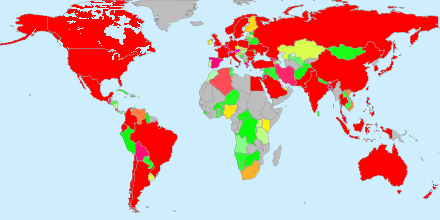
\includegraphics[scale=0.6]{images/prefixhj.png}
    \caption{Result of the China Telecommunications hijack in 2010. Countries in red have more than 200 prefixes impacted. \cite{prefixhj}}
    \label{fig:prefixhj}
\end{figure}
\newpage

In 2010 a China Telecommunications Corporation started to announce about 37000 unique prefixes by mistake\cite{prefixhj}. Figure \ref{fig:prefixhj} illustrates the significant portion of the world that was affected by this mistake. Another example of a BGP hijack originates from 2008, where Pakistani Telecom accidentaly announced a subnet of a prefix owned by YouTube. Due to the nature of BGP, this invalid route was spread over the global Internet, causing availability issues for YouTube all over the world\cite{youtubehack}.\par

\section{Scope}\label{sec:scope}
This project aims to detect BGP hijacks near real-time, with a focus on Dutch IP space. Thereby solely using public available information without disclosing any prefix information to third parties. Some papers talk about BGP leaks \cite{hu2007accurate}, this means that routes from clients are send to peer routers, so they will advertise these routes to the uplink routers. This will create a false positive because the AS-path is different and for some ASNs not the shortest. This could be detected as a hijack, but it is desired behavior. Detecting BGP leaks is out of scope for this project.

\section{Layout}\label{sec:layout}
The layout of this paper is as follows. Existing work will be discussed first, whereafter the problem will be discussed in chapter \ref{ch:problem}. After a research question has been defined, a new model to detect BGP hijacks is described in chapter \ref{ch:model}. Next, experimentations are discussed and their results reviewed. This report will conclude with a wrap-up of the results, whereafter there'll be a final discussion on future work.

\section{Terminology}\label{sec:terminology}
While reading this paper some terms will occur frequently. It is important to know what these terms mean in this paper. When the term prefix is mentioned it means an IP network block written in the Classless Inter-Domain Routing (CIDR) notation. i.e. 145.92.0.0/16. A subnet is a small part of a specific prefix referred to in the text. i.e. 145.92.160.64/26 is a subnet from prefix 145.92.0.0/16. The term supernet is used to refer to a larger network than the specific prefix referred to in the text. i.e. 145.80.0.0/12 is a supernet for prefix 145.92.0.0/16. BGP routers containing the full BGP routing table don't need a default route. They know how to route traffic to every network because they have mostly directly connected neighbors they peer with. The 'zone' these routers are in, is called the Default Free Zone (DFZ). 
